% !TEX root = ../agglo_clust_review.tex

\section{Introduction}
In computer vision, the partitioning of weighted graphs has been successfully applied to such tasks as image segmentation, object tracking and pose estimation. 
Most graph clustering methods work with positive edge weights only, which can be interpreted as similarities or distances between the nodes. These methods are parameter-based and require users to specify the desired numbers of clusters or a termination criterion (e.g. spectral clustering or iterated normalized cuts) or even to add a seed for each object  (e.g. seeded watershed or random walker).  

Other graph clustering methods work with so-called \emph{signed graphs}, which include both positive and negative edge weights corresponding to attraction and repulsion between nodes. The advantage of signed graphs over positive-weighted graphs is that balancing attraction and repulsion allows us to perform the clustering without defining additional parameters. This can be done optimally by solving the so-called \emph{multicut optimization} or \emph{correlation clustering} problem \cite{kappes2011globally,chopra1991multiway}. This problem is NP-hard, but approximate solvers have already been proposed \cite{beier2016efficient}. Besides, the general problem of graph partitioning can be solved approximately by greedy agglomerative clustering \cite{keuper2015efficient,levinkov2017comparative,wolf2018mutex,kardoostsolving}. 


Agglomerative clustering algorithms for signed graphs have clear advantages: they are parameter-free and efficient. Despite the fact that there exists a variety of these algorithms, no overarching study has so far been made to compare their robustness and efficiency or to provide guidelines for matching an algorithm to the partitioning problem at hand. 


In this paper, we propose a novel theoretical framework that generalizes over agglomerative algorithms for signed graphs by linking them to hierarchical agglomerative clustering on positive-weighted graphs \cite{lance1967general}. This framework defines an underlying basic algorithm and allows us to explore its combinations with different linkage criteria and \emph{cannot-link constraints}. 
We then formally prove that some of the combinations correspond to existing clustering algorithms and introduce new algorithms for combinations which have not been explored yet.

We evaluate and compare these algorithms on \emph{instance segmentation} - a computer vision task of assigning each pixel of an image to an object instance. 
We use a CNN to predict the edge weights of a graph such that each node represents a pixel of the image, similarly to \cite{liu2018affinity,lee2017superhuman,wolf2018mutex}, and provide these weights as input to the algorithms in our framework (see Fig. \ref{fig:intro_figure}). 

\begin{figure*}[t]
\centering
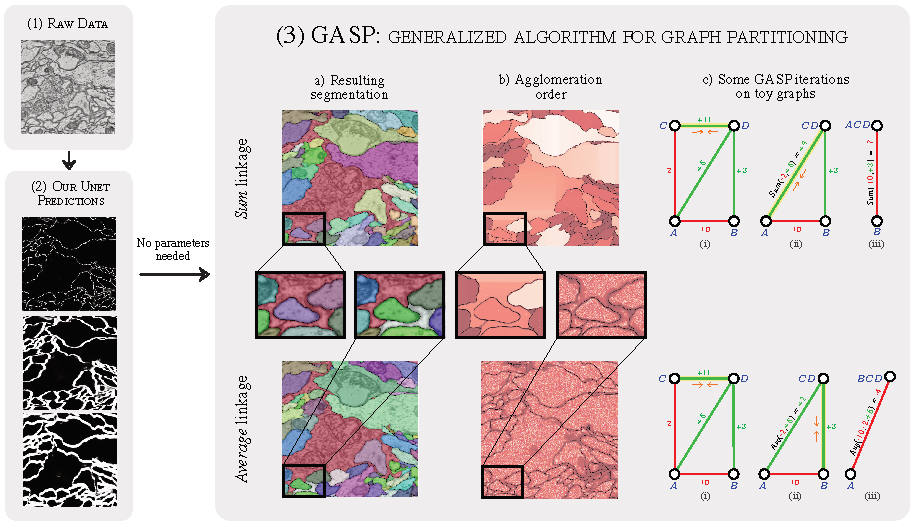
\includegraphics[width=0.9\textwidth]{figs/intro_image_v3.pdf} % left bottom right top
\caption{ Pipeline description: \textbf{(1)} Raw data from the CREMI 2016 neuron-segmentation challenge. \textbf{(2)} Some short- and long-range predictions of our CNN model, where white pixels represent boundary evidence. \textbf{(3)} Outputs of two agglomerative algorithms included in our proposed generalized clustering framework, with \emph{Sum} and \emph{Average} linkage criteria. The final clustering / instance segmentation is shown in 3a, overlaid with the raw image.  The  agglomeration order in 3b shows which pairs of neighboring pixels were merged first (white), later on (brown/red), or never (black). (\textbf{4}) Some iterations of \algname{} on toy graph examples with attractive/positive (green) and repulsive/negative (red) interactions. At each iteration, the yellow edge with highest interaction is contracted (orange arrows), until only negative edges are left in the graph.
\label{fig:intro_figure}}
\end{figure*}


With our comparison experiments, performed both on 2D urban scenes from the CityScapes dataset and 3D electron microscopy image volumes of neurons, we evaluate the properties of the algorithms in our framework, focusing on their efficiency, robustness and tendency to over- or under-cluster.
We show that one of the new algorithms derived from our framework, based on an average linkage criterion, outperforms the previously known agglomeration methods expressed in the framework and 
it achieves competitive performance on CityScapes and the challenging CREMI 2016 segmentation benchmark.

In Sec. \ref{sec:spectral_clust}, we also show how \algname{} outperforms spectral clustering methods on the task of neuron segmentation and how on synthetic graphs it achieves similar scores to a recently proposed spectral method for signed graphs.

% Our code is available at \url{https://github.com/abailoni/GASP}.


